%========================================
% Beamer "Singapore" Theme Template
%========================================
\documentclass[aspectratio=169]{beamer}

% THEME
\usetheme{Singapore}            % clean sidebar theme

% COLORS & FONTS (tweak as desired)
\definecolor{brand}{RGB}{45,110,191}
\definecolor{accent}{RGB}{5,155,192}
\definecolor{hrgray}{RGB}{100,100,100}
\setbeamercolor{structure}{fg=brand}
\setbeamercolor{title}{fg=hrgray}
\setbeamercolor{subtitle}{fg=brand}
\setbeamercolor{author}{fg=hrgray}
\setbeamercolor{date}{fg=hrgray}
\setbeamercolor{frametitle}{fg=hrgray}
\setbeamercolor{block title}{fg=white,bg=brand}
\setbeamercolor{block body}{bg=black!2}
\usepackage{lmodern}
\usefonttheme{professionalfonts}

\usepackage{etoolbox}
\usepackage[T1]{fontenc}
\usepackage[utf8]{inputenc}
\usepackage{microtype}
\usepackage{graphicx}
\usepackage{makecell}
\usepackage{tikz}
\usepackage{xcolor}

% tables
\usepackage{multirow} 
\usepackage[table]{xcolor}
\usepackage{makecell}
\usepackage{booktabs}
\usepackage{colortbl}

\newcolumntype{C}[1]{>{\centering\arraybackslash}m{#1}} % Generic centered column
\newcolumntype{N}{>{\columncolor{gray!20}\centering\arraybackslash}m{0.1cm}} % Narrow, grey, centered

\setbeamertemplate{navigation symbols}{} % optional: hide nav icons
\setbeamertemplate{frametitle continuation}{}

\setbeamertemplate{footline}{
  \leavevmode
  \hbox{
    % LEFT: logo
    \begin{beamercolorbox}[wd=.5\paperwidth,ht=3ex,dp=1ex,left]{author in head/foot}
      \hspace{0.8ex}{
\includegraphics[height=0.5cm]{gw_logo.png}} % gwu branding
    \end{beamercolorbox}%
    % RIGHT: page number
    \begin{beamercolorbox}[wd=.5\paperwidth,ht=3ex,dp=1ex,right]{date in head/foot}
      \insertframenumber{} / \inserttotalframenumber\hspace{2ex}
    \end{beamercolorbox}%
  }
  \vskip0pt
}

% METADATA
\title{Chief AI Officer Report}
\subtitle{Update 1}
%\subtitle{AI Measurement in the Real World}
\author[Your Name]{\textbf{Patrick Hall}}
\institute{jphall@gwu.edu}
\date{\today}

% handle URLs/links
\PassOptionsToPackage{hyphens}{url}\usepackage{hyperref}
\urlstyle{same}
\hypersetup{% customize link colors
    colorlinks=true,
    urlcolor=[rgb]{0.0196, 0.6078, 0.7529},
    linkcolor=[rgb]{0.17647, 0.388, 0.749},
    citecolor=[rgb]{0.0196, 0.6078, 0.7529}}

% Chicago citations and bibliography
\setbeamertemplate{bibliography item}[text]
\usepackage[authordate]{biblatex-chicago}
\addbibresource{references.bib}
\setlength{\bibitemsep}{0.5\baselineskip}
\AtBeginBibliography{\scriptsize}
\renewcommand\UrlFont{\sffamily}


\begin{document}

%-------------------------
\begin{frame}
  \titlepage
  % Title slide with centered, semi-transparent PDF watermark
  \begin{tikzpicture}[remember picture,overlay]
    \node[opacity=0.1] at (current page.center)
      {
\includegraphics[width=0.55\paperwidth]{gw_logo.png}}; %gwu brnading 
      % try width=0.9\paperwidth or height=0.6\paperheight to taste
  \end{tikzpicture}
\end{frame}

%-------------------------
\begin{frame}{Agenda}
  \tableofcontents
\end{frame}

%-------------------------
\section{First Steps}
%-------------------------

\begin{frame}{First Steps}

    \begin{itemize}\small
        \item Chaired alumni \href{https://connect.gwu.edu/site/Calendar?id=131102&view=Detail}{panel} on AI. 
        \item Hosted inaugural GWSB AI case competition.
        \item Co-chairing operations subcommittee for university president's strategic AI mapping exercise:
        \begin{itemize}
            \item Drafted a comprehensive survey instrument to collect data from university business units. 
            \item Unlocked access to data and insights across schools, departments, and units. 
        \end{itemize}
        \item Socialized participatory GWSB AI Forum--90+ faculty and staff signups to date. 
        \item Discussing approval of AI coding agents for teaching purposes with GW IT. 
        \item Conducted initial analysis of university AI and data policies.
    \end{itemize}
  
\end{frame}

\subsection*{GWSB AI Case Competition}

\begin{frame}{GWSB AI Case Competition}

\begin{columns}

    \column{0.5\textwidth}

        \begin{center}
            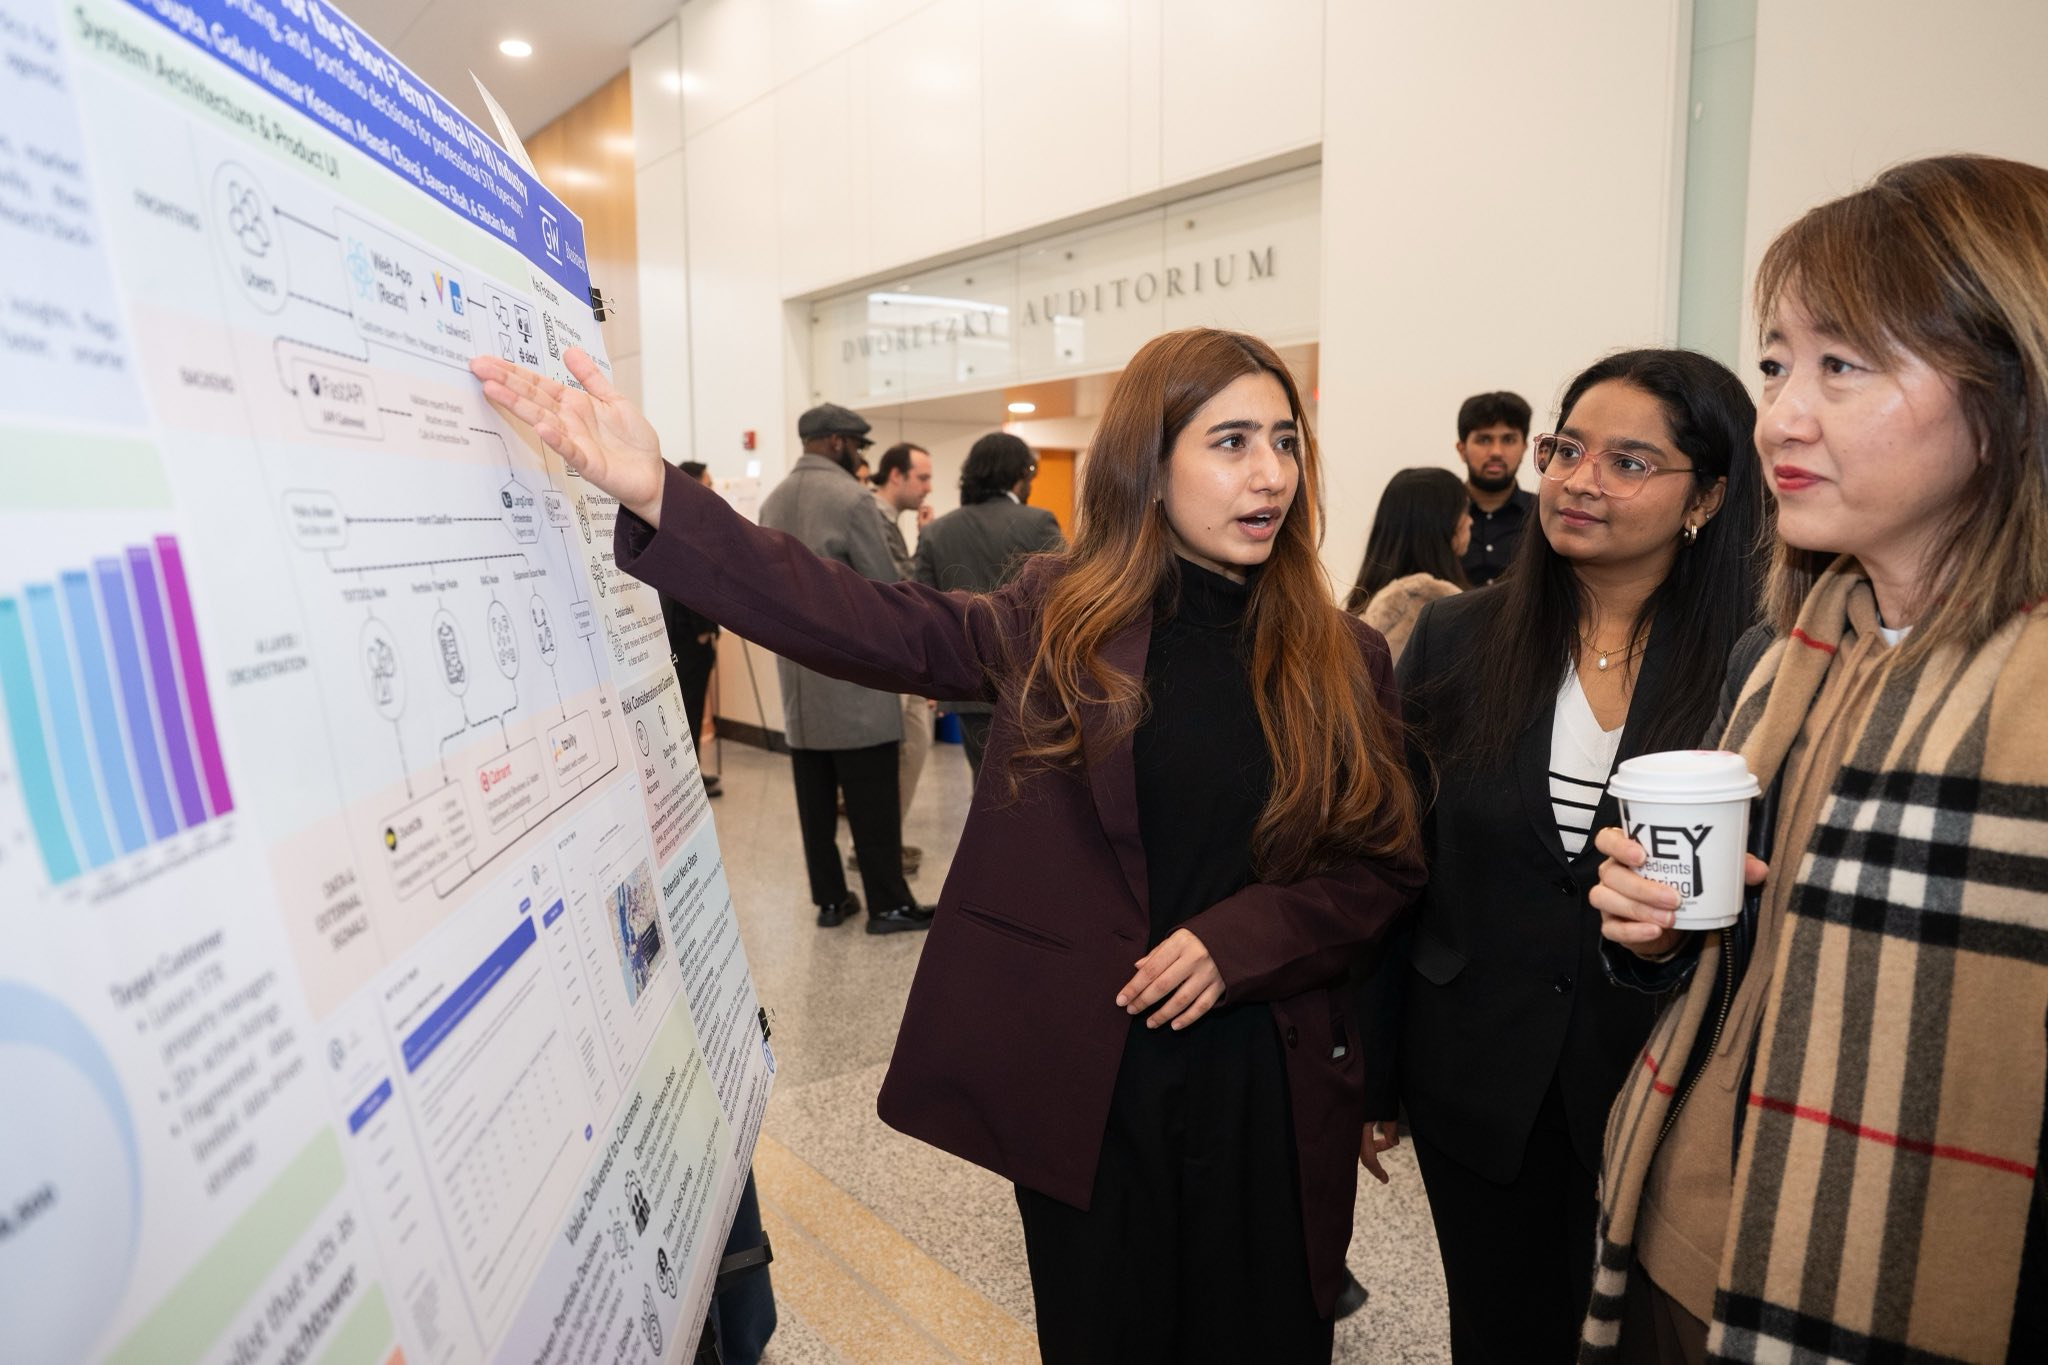
\includegraphics[width=0.87\linewidth, keepaspectratio]{GWSB_AI_Case_Competition_2025_LF_28.jpg}\\
            \scriptsize{Current MSBA students explain their AI project to an MSBA alumna that works in banking analytics.} 
        \end{center}

    \column{0.5\textwidth}
        \begin{itemize}
            \item 14 groups (61 students) created and presented AI agents.
            \item Corporate judges from Capital One, EY, FI Consulting (local), and Mizuho.
            \item Winners included fraud detection, financial analysis, and travel orchestration agents. 
            \item 100+ attendees, multiple \href{https://www.linkedin.com/feed/update/urn:li:activity:7403912440557518848/}{social posts}, and strong interest in next semester's competition. 
        \end{itemize}

\end{columns}

\end{frame}

%-------------------------
\section{Next Steps}
%-------------------------

\begin{frame}{Next Steps}

    \begin{table}[h!]
    \centering
    \begin{tabular}{|l|l|l|}
    \hline
    \textbf{Step} & \textbf{Tentative Date}  & \textbf{Notes}  \\ \hline
    \textbf{GWSB AI Forum} & 15 Jan. 2025 & \makecell[l]{\tiny{Slack and email forum to gather participatory input}\\[-3pt]\tiny{from GWSB faculty and staff}.} \\ \hline
    \textbf{Policy Analysis} & 15 Jan. 2025 & \tiny{Analysis of existing GWU AI policies/peer benchmarking.} \\ \hline
    \textbf{AI Awards Program} & 15 Feb. 2025 & \tiny{Process and criteria for GWSB AI awards program.} \\ \hline
    \textbf{GWSB AI Inventory} & 15 Mar. 2025 & \tiny{Documentation of existing GWSB AI work.} \\ \hline
    \textbf{Human-AI Teaming Seminar} & 15 Apr. 2025 & \tiny{GWSB seminar on effective ways to work \textit{with} AI.} \\ \hline
    \textbf{AI Executive Education} & 15 May 2025 & \tiny{Curriculum for CAIOs, targeting DC market.} \\ \hline
    \textbf{Responsible Use Policy} & 15 Jun. 2025 & \tiny{Define rules-of-the-road for AI usage at GWSB.} \\ \hline
    \end{tabular}
    \end{table}

\end{frame}

%-------------------------
\section{Policy Analysis}

\subsection*{Existing Policies}

\begin{frame}{Existing Policies}

    \begin{itemize}
        \item Existing policies:
        \begin{itemize}
            \item GWU IT policies address approved tools, security, and data classification. 
            \item Libraries \& Academic Innovation guidance provides resources for teaching. 
            \item Office of Ethics, Compliance, and Risk policies address data privacy, digital identity, and overall responsible technology use. 
            \item Office of the Provost provides guidelines for faculty. 
            \item The Data Privacy Office provides in-depth policies and guidance for privacy. 
        \end{itemize}
        \item Perceived gaps: nondiscrimination, responsible AI.
        \item Created basic public \href{https://github.com/jphall663/gwsb_caio}{knowledge base} and interactive NotebookLM \href{https://notebooklm.google.com/notebook/d6709e69-032a-427c-bc07-8f23bf19c184}{tool} for AI-guided policy Q\&A.
    \end{itemize}

\end{frame}

\subsection*{Analysis}

\begin{frame}{\small{Existing Policies--Topic Word Cloud}}

    \begin{center}
        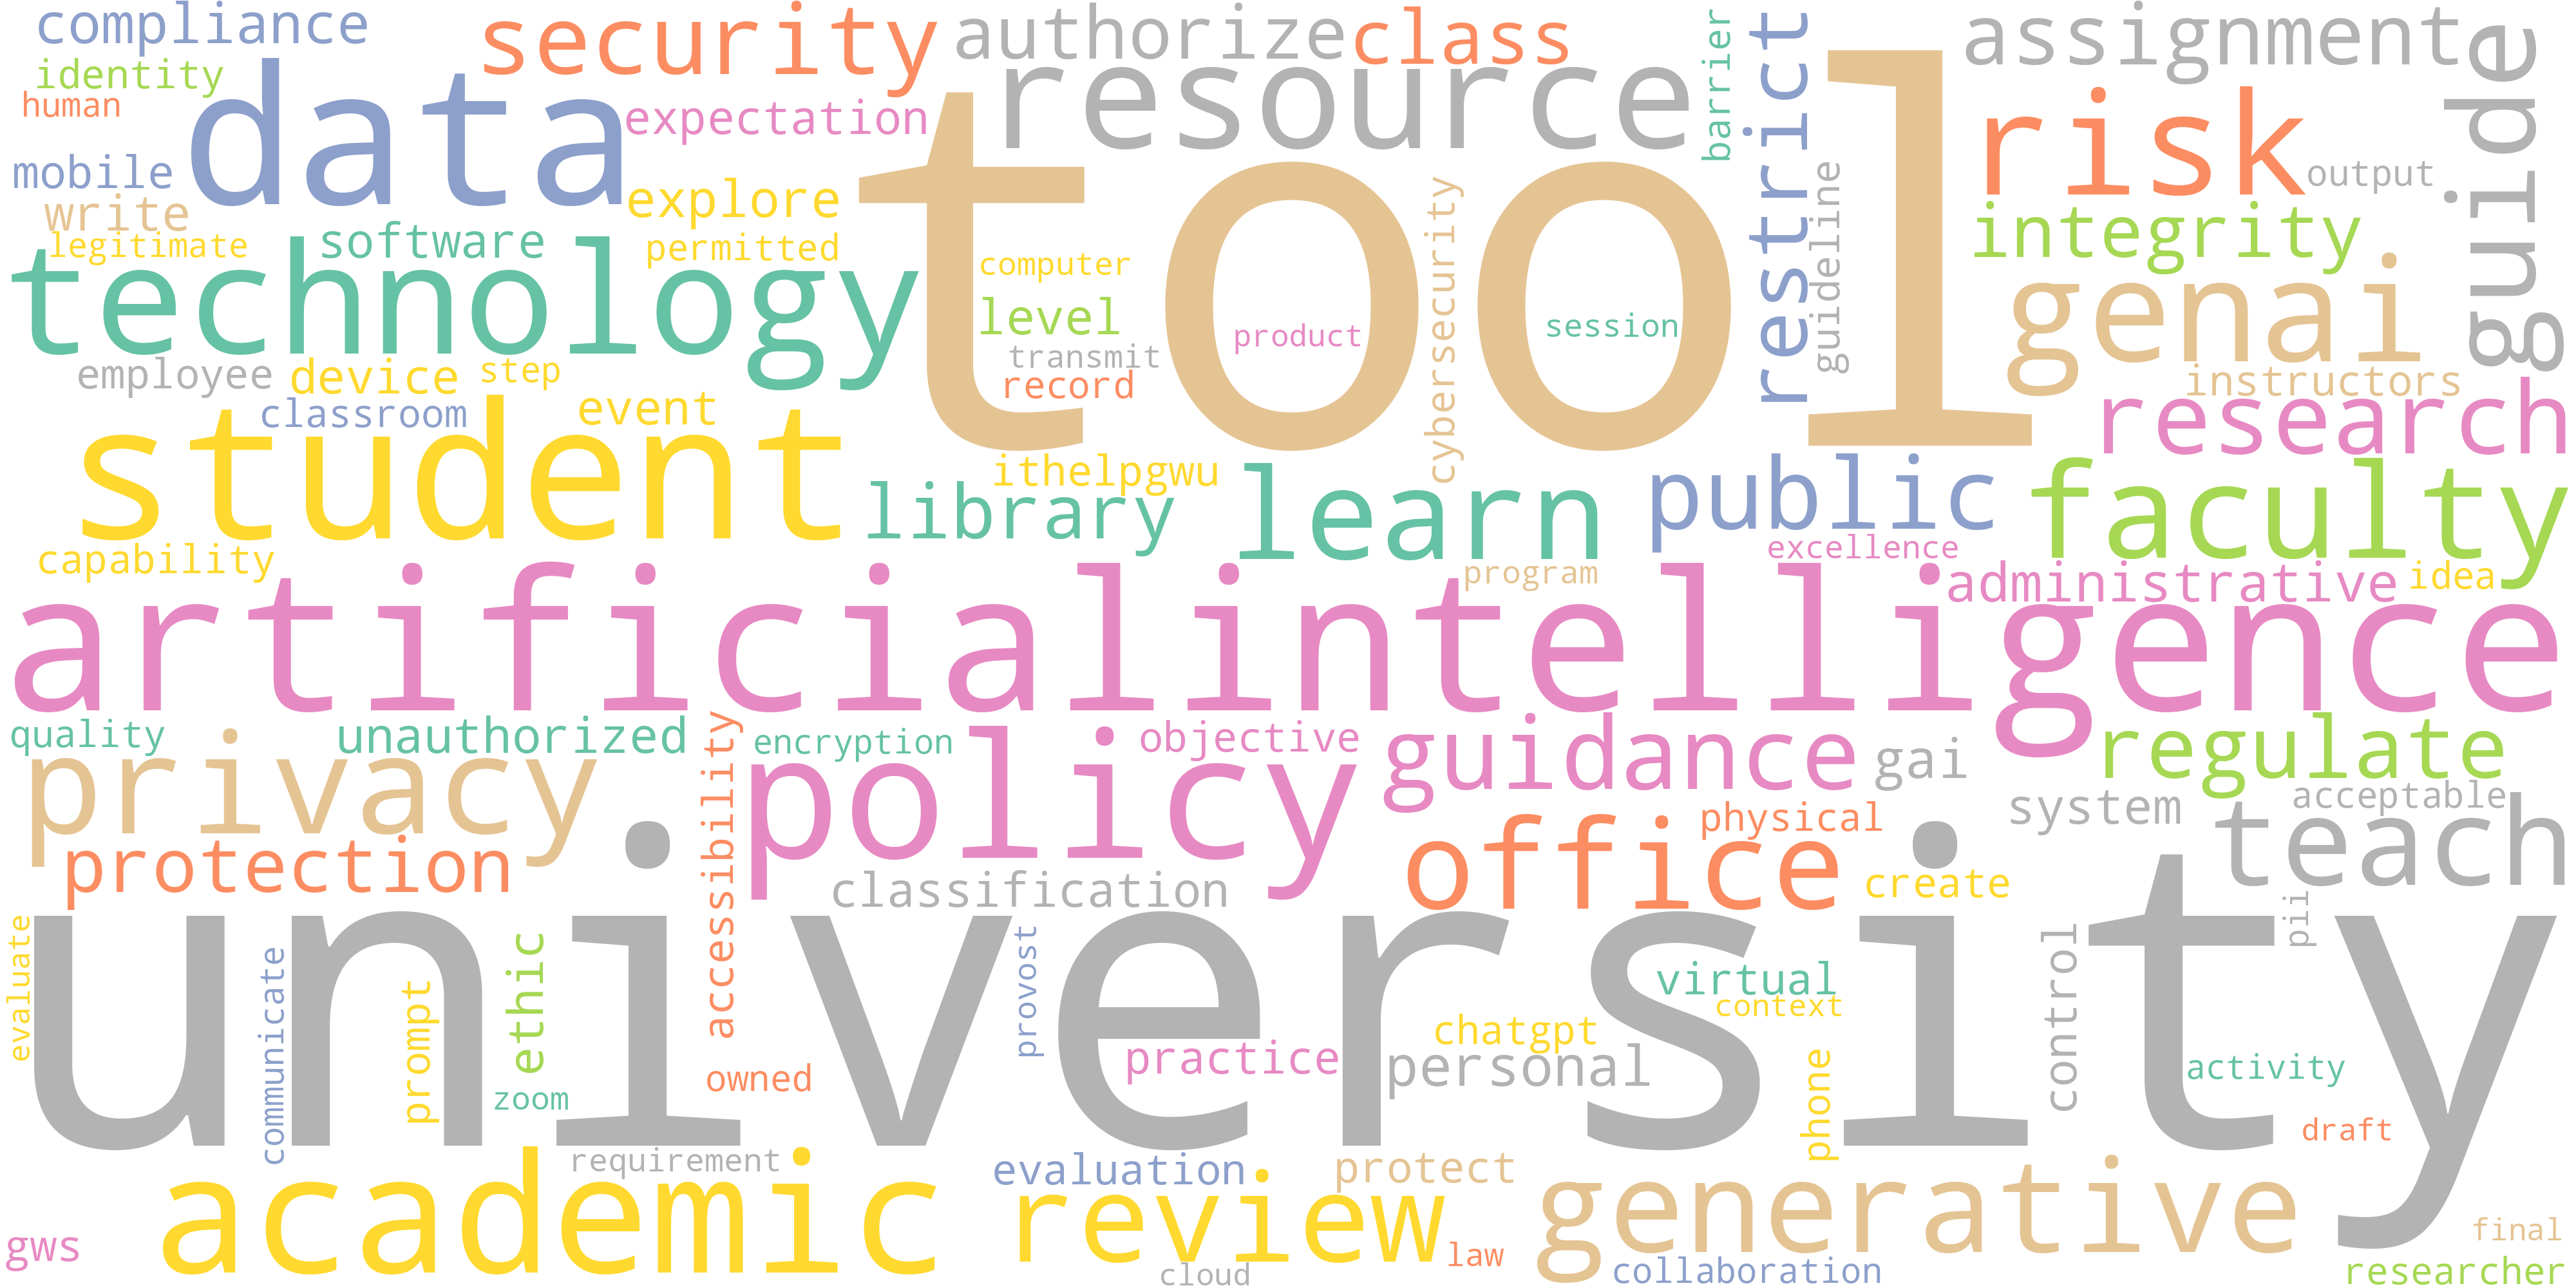
\includegraphics[width=0.87\linewidth, keepaspectratio]{existing_policy_key_word_cloud_hi_4k.png}\\
        \vspace{5pt}\scriptsize{Top keywords across existing GWU AI policies.} 
    \end{center}

\end{frame}

\begin{frame}{\small{Existing Policies--Topic Clusters}}

    \begin{center}
        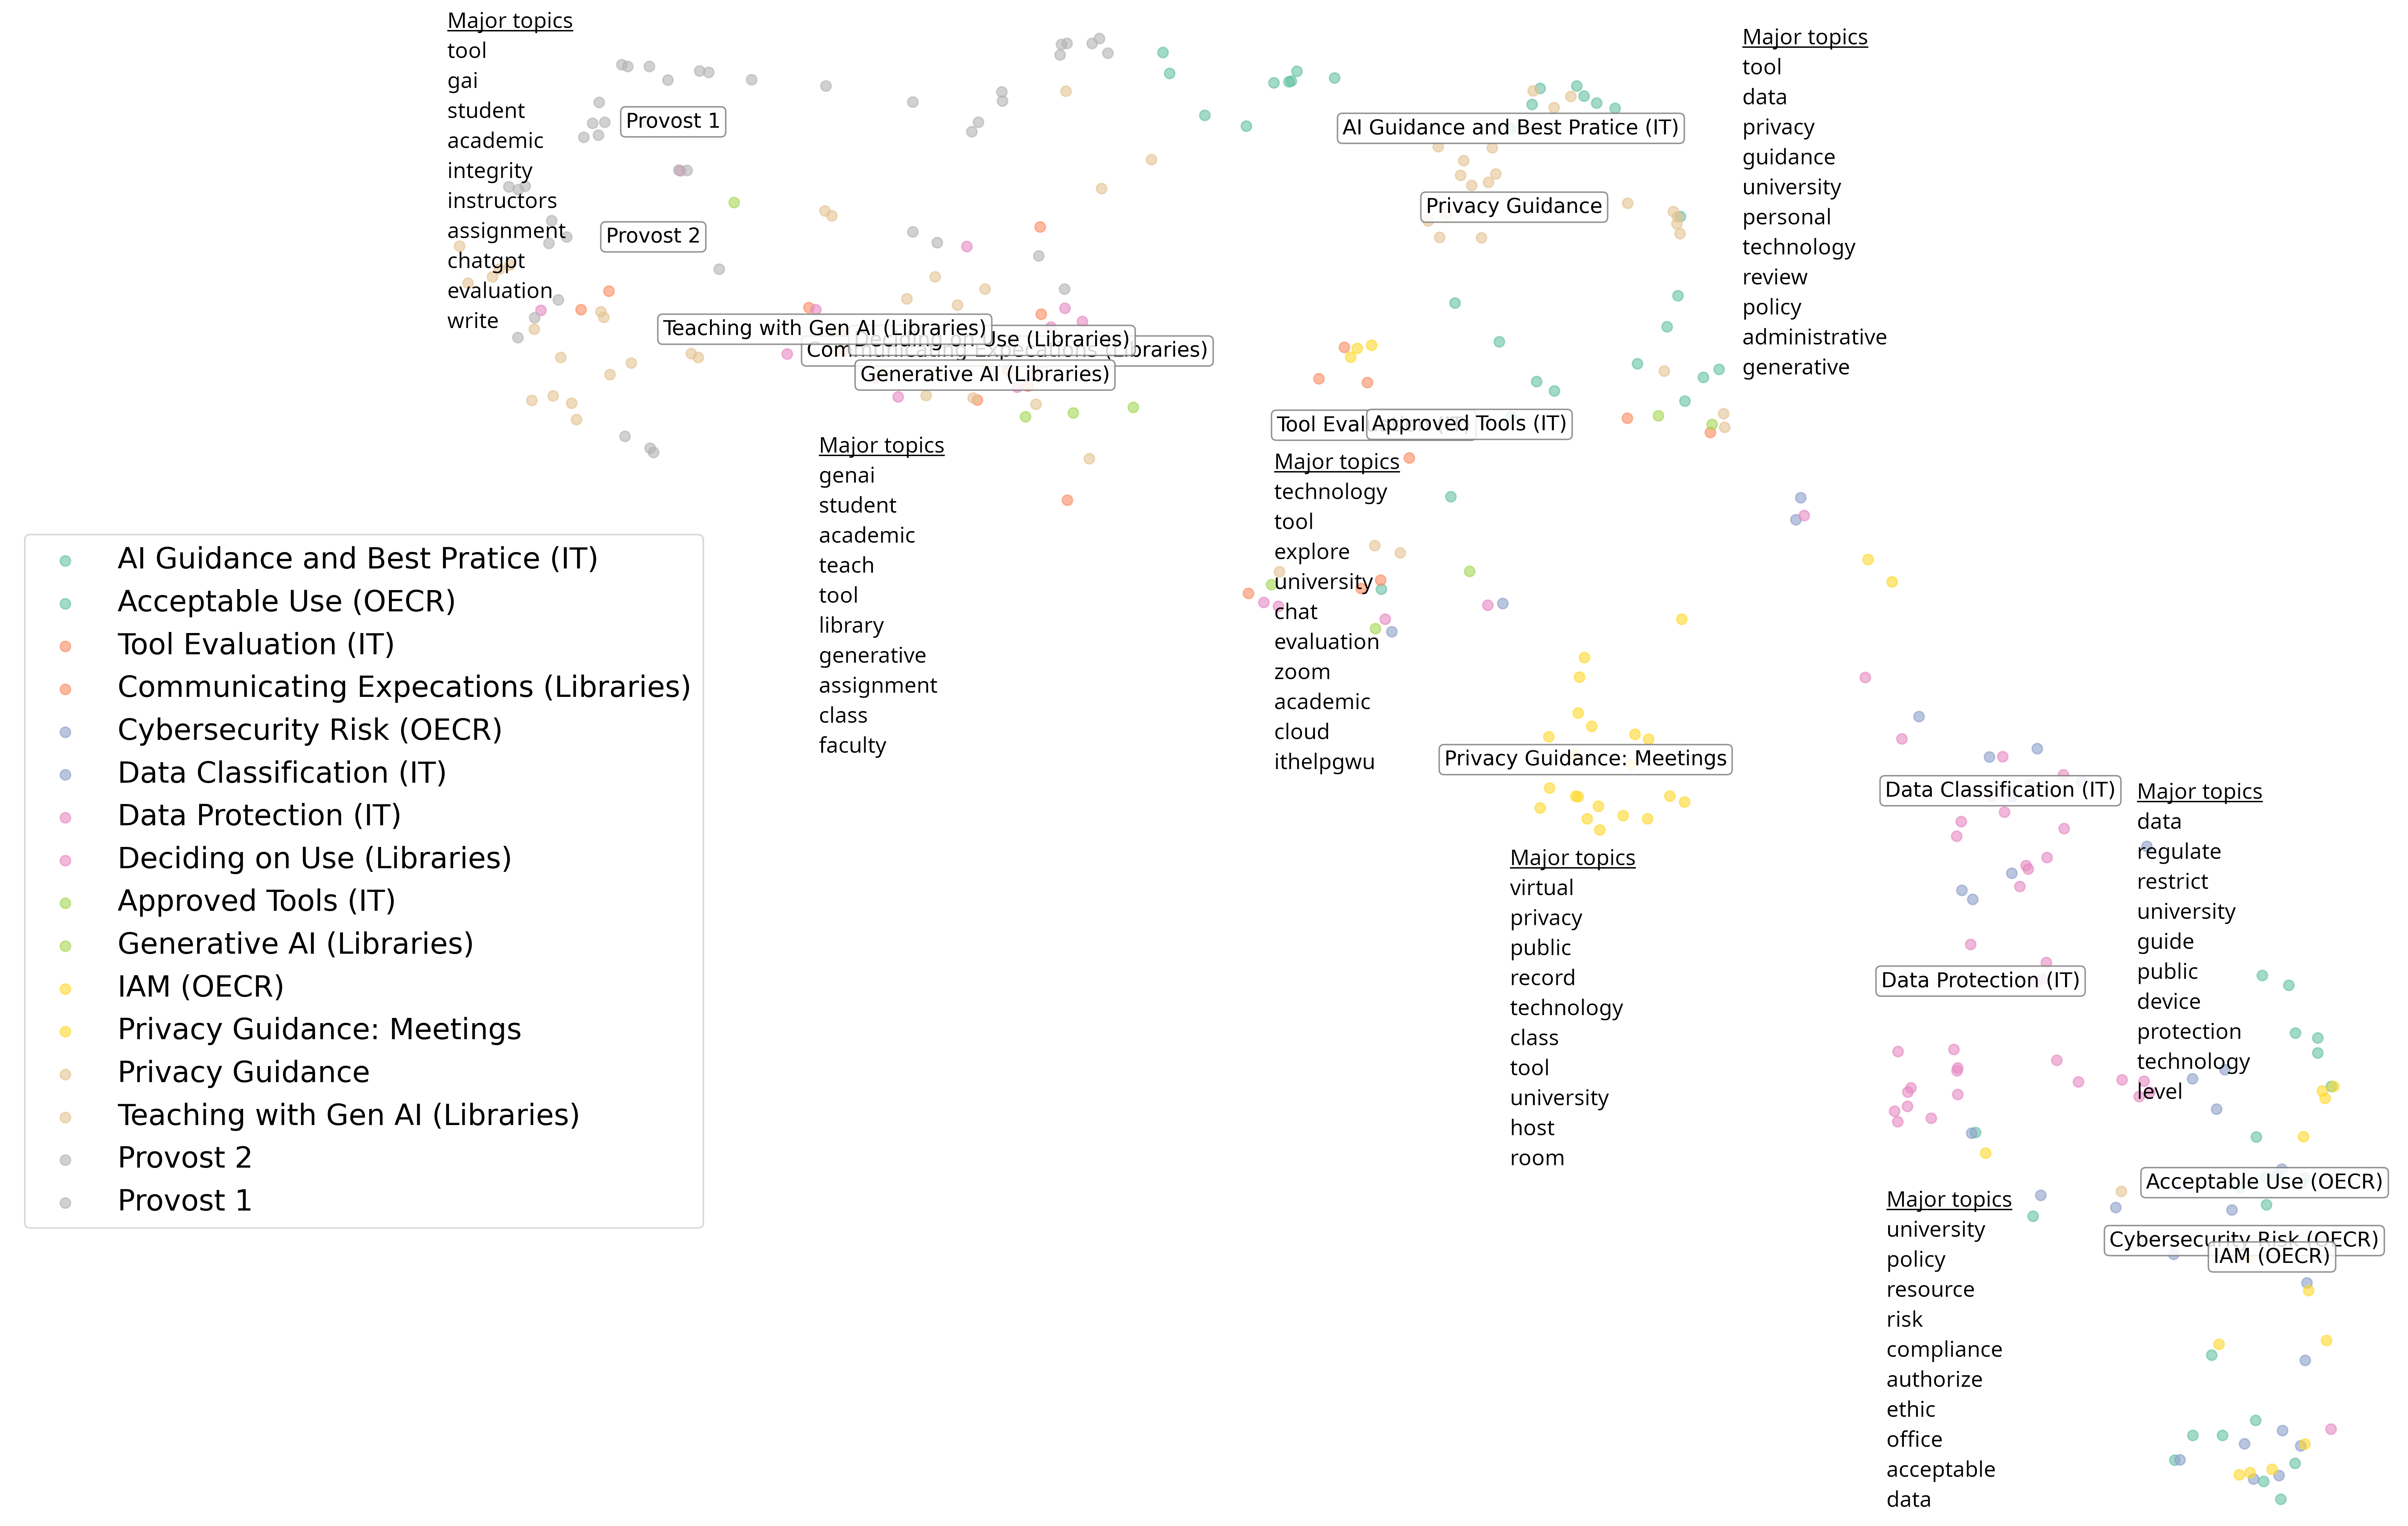
\includegraphics[height=0.47\linewidth, keepaspectratio]{doc_clus_legend_annotated_crop.png}\\
        \vspace{5pt}\scriptsize{Document clusters and their associated keywords for existing GWU AI policies.} 
    \end{center}

\end{frame}

%-------------------------

\end{document}
